\documentclass[aspectratio=43]{beamer}
% use this instead for 16:9 aspect ratio:
%\documentclass[aspectratio=169]{beamer}
% supported acpect ratios  1610  169 149 54 43 (deault) 32

\usepackage[english]{babel} 
\usepackage[utf8]{inputenc}
\usepackage[T1]{fontenc} 	
\usetheme{ETHbeamer}
\usepackage{graphicx} 
	\graphicspath{ {images/}{plots/} }
\usepackage{subcaption}
\usepackage[sort,comma,numbers]{natbib}
	\bibliographystyle{unsrtnat}
	
\colorlet{ETHcolor1}{ETHc}
\colorlet{ETHcolor2}{ETHh}

\author[LQS]{Lefkopoulos Vasileios, Qi Shuaixin, Signer Matteo}

\title{Decision-making in the social force model for an evacuation process}

\date{18-12-2017}

% uncomment if you do not want to use a department logo
\deplogofalse


\begin{document}


\titleframe


\begin{frame}{Outline}
	\begin{enumerate}
		\item Introduction
		\smallskip
		\item Motivation
		\smallskip
		\item Research Questions
		\smallskip
		\item Model
		\smallskip
		\item Simulations
		\smallskip
		\item Summary
	\end{enumerate}
\end{frame}


\begin{frame}{Introduction}
	\pause
	
	Evacuation scenarios are (unfortunately) common occurrences.
	
	\bigskip
	\pause
	
	Some examples:
	\begin{itemize}
		\item Jamaraat Bridge, Saudi Arabia, 2006. \\
		\item Love Parade, Germany, 2010. \\
		\item Grenfell Tower, UK, 2017. \\
	\end{itemize}

	\begin{figure}
		\centering
		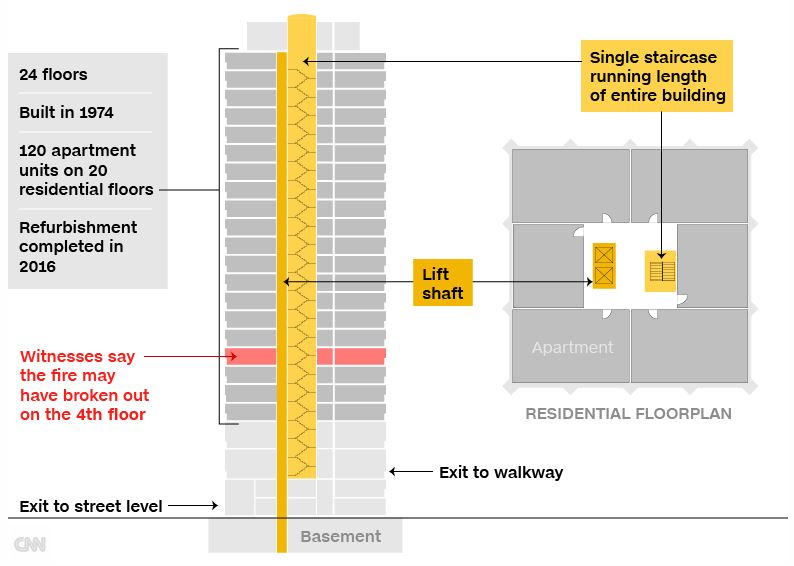
\includegraphics[width=0.5\linewidth]{grenfell_tower.jpg}
	\end{figure}
\end{frame}


\begin{frame}{Motivation}
	\pause
	
	\begin{itemize}
		\item Understand the crowd dynamics in a simple evacuation scenario. \\
		\bigskip
		\item Minimize the danger and optimize with respect to safety. \\
		\bigskip
		\pause
		\item Many proposed models ignore the decision-making of the agents. \\
		\bigskip
		\item We integrated the decision-making into a well-known model.
	\end{itemize}
\end{frame}


\begin{frame}{Model}
	\pause
	
	The agent-based \emph{social force} model, proposed by \citet{Helbing2000}, with modifications from \citet{Zainuddin2010} and \citet{Wang2016}.
	
	\begin{minipage}{.5\textwidth}
			\centering
			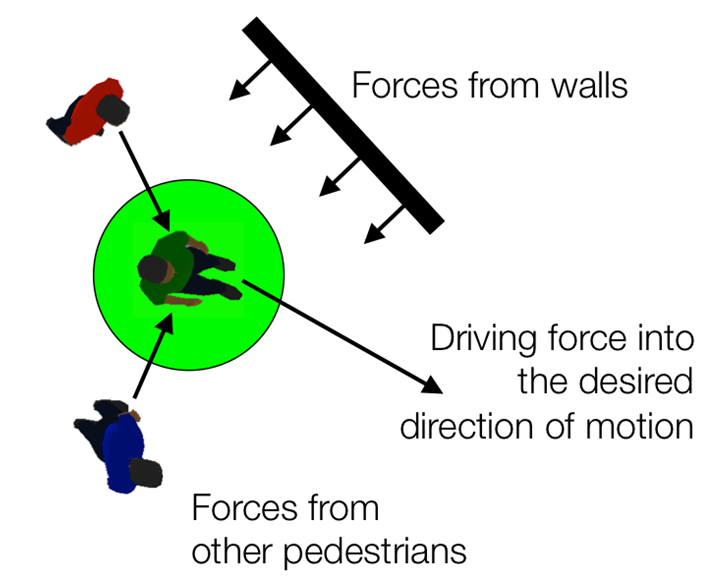
\includegraphics[width=0.9\linewidth]{social_force.png}
	\end{minipage}\begin{minipage}{.5\textwidth}
		\centering
		\includegraphics[width=0.9\linewidth]{{demo_P-0.4_0200_4.000}.eps}
	\end{minipage}
\end{frame}


\begin{frame}{Model -- Equations of Motion}
	\begin{equation*}
		m_i \frac{d\bm{v}_i}{dt}(t) = m_i \frac{\bm{v}_i^0(t) -\bm{v}_i(t)}{\tau_i} + \sum_{j(\neq i)}^{}\bm{f}_{ij}(t) + \sum_{w}^{}\bm{f}_{iw}(t) + \sum_{k}^{}\bm{f}_{ik}(t)
	\end{equation*}
	
	\vfill
	
	\begin{itemize}
		\item $m_i \frac{d\bm{v}_i}{dt}(t)$: total force
		\smallskip
		\item $ m_i \frac{\bm{v}_i^0(t) -\bm{v}_i(t)}{\tau_i}$: driving force
		\smallskip
		\item $\bm{f}_{ij}(t)$: interaction force between agents
		\smallskip
		\item $\bm{f}_{iw}(t)$: interaction force between agents and walls
		\smallskip
		\item $\bm{f}_{ik}(t)$: interaction force between agents and exits
	\end{itemize}
\end{frame}


\begin{frame}{Model -- Forces}
	\begin{equation*}
	\begin{split}
		\bm{f}_{ij}(t) & = \bm{f}_{ij}^{psych}(t) + \bm{f}_{ij}^{push}(t) + \bm{f}_{ij}^{frict}(t) \\[0.5em]
		\bm{f}_{iw}(t) & = \bm{f}_{iw}^{psych}(t) + \bm{f}_{iw}^{push}(t) + \bm{f}_{iw}^{frict}(t) \\[0.5em]
		\bm{f}_{ik}(t) & =\bm{f}_{ik}^{psych}(t)
	\end{split}
	\end{equation*}
	
	\vfill
	
	\begin{itemize}
		\item $\bm{f}^{psych}(t)$: psychological force
		\smallskip
		\item $\bm{f}^{push}(t)$: body force
		\smallskip
		\item $\bm{f}^{frict}(t)$: sliding friction force
	\end{itemize}
\end{frame}


\begin{frame}{Model -- Velocity}
	\begin{equation*}
		\bm{v}_i^0(t) = (1-p_i) \nu_i^0 \bm{e}_i^0(t) + p_i \bar{\bm{v}}_i^0(t)
	\end{equation*}
	
	\vfill
	
	\begin{itemize}
		\item $\nu_i^0$: desired velocity
		\smallskip
		\item $\bm{e}_i^0(t)$: desired direction
		\smallskip
		\item $p_i$: panic level
		\smallskip
		\item $\bar{\bm{v}}_i^0(t)$: average velocity of surrounding agents
	\end{itemize}
\end{frame}


\begin{frame}{Model -- Decision-making}
	\begin{equation*}
	\begin{split}
		\bm{e}_i^0(t) & = - \nabla d_{k_i^*}(\bm{r}_i) \\
		k_i^*(t) & = indmax\{ (1+g_i) U_{ik_i^*}(t) \,, \max_k\left(U_{ik}(t)\right) \} \\
		U_{ik}(t) & = \exp\left( -l_i d_{ik}^{unc}(t) E_i \right) \left(1-\alpha_i\left(\frac{r_k(t)}{\max_k\left(r_k(t)\right)}\right)^{\beta_i}\right) \delta(\varphi_{ik}(t))
	\end{split}
	\end{equation*}
	
	Decision-making process:
	\begin{enumerate}
		\item Each agent has a field of view $[180^{\circ},360^{\circ}]$, depending on the excitement factor $E_i \in [0,1]$. \\
		\item He calculates the value $U_{ik}(t)$ of the visible exits, according to the distance and congestion of each exit.
		\item He chooses the exit $k_i^*$ with the highest value and changes his direction $\bm{e}_i^0(t)$ accordingly.
	\end{enumerate}
\end{frame}


\begin{frame}{Research Questions}
	\pause
	
	\begin{enumerate}
		\item How does the \emph{desired velocity} affect the behaviour of the agents during the evacuation? \\
		\smallskip
		\item How does the \emph{desired velocity} affect the evacuation time? \\
		\smallskip
		\pause
		\item How does the \emph{panic level} affect the behaviour of the agents during the evacuation? \\
		\smallskip
		\item How does the \emph{panic level} affect the evacuation time? \\
		\smallskip
		\pause
		\item How does the \emph{excitement factor} affect the behaviour of the agents during the evacuation?
	\end{enumerate}
\end{frame}


\begin{frame}{Simulations -- Desired Velocity}
	\pause
	
	For a desired velocity of $\nu_i^0 = 2.22 ms^{-1}$:
	
	\begin{figure}
		\centering
		\includegraphics[width=.9\linewidth]{{demo_V-2.22_0500_5.000}.eps}
		\caption{$t = 5s$}
	\end{figure}
\end{frame}


\begin{frame}{Simulations -- Desired Velocity}
	For a desired velocity of $\nu_i^0 = 2.22 ms^{-1}$:
	
	\begin{figure}
		\centering
		\includegraphics[width=.9\linewidth]{{demo_V-2.22_1000_10.000}.eps}
		\caption{$t = 10s$}
	\end{figure}
\end{frame}


\begin{frame}{Simulations -- Desired Velocity}
	For a desired velocity of $\nu_i^0 = 2.22 ms^{-1}$:
	
	\begin{figure}
		\centering
		\includegraphics[width=.9\linewidth]{{demo_V-2.22_1500_15.000}.eps}
		\caption{$t = 15s$}
	\end{figure}
\end{frame}


\begin{frame}{Simulations -- Desired Velocity}
	For a desired velocity of $\nu_i^0 = 2.22 ms^{-1}$:
	
	\begin{figure}
		\centering
		\includegraphics[width=.9\linewidth]{{demo_V-2.22_2000_20.000}.eps}
		\caption{$t = 20s$}
	\end{figure}
\end{frame}


\begin{frame}{Simulations -- Desired Velocity}
	For a desired velocity of $\nu_i^0 = 2.22 ms^{-1}$:
	
	\begin{figure}
		\centering
		\includegraphics[width=.9\linewidth]{{demo_V-2.22_2500_25.000}.eps}
		\caption{$t = 25s$}
	\end{figure}
\end{frame}


\begin{frame}{Simulations -- Desired Velocity}
	For a desired velocity of $\nu_i^0 = 2.22 ms^{-1}$:
	
	\begin{figure}
		\centering
		\includegraphics[width=.9\linewidth]{{demo_V-2.22_3000_30.000}.eps}
		\caption{$t = 30s$}
	\end{figure}
\end{frame}


\begin{frame}{Simulations -- Desired Velocity}
	For a desired velocity of $\nu_i^0 = [1.35,2.25]ms^{-1}$:
	
	\begin{figure}
		\centering
		\includegraphics[width=.8\linewidth]{{demo_V}.eps}
	\end{figure}
\end{frame}


\begin{frame}{Research Questions -- Desired Velocity}
	\pause
	
	\begin{itemize}
		\item How does the desired velocity affect the behaviour of the agents during the evacuation? \\
		\smallskip
		\emph{A higher desired velocity caused the agents to try and move with a higher velocity.} \\
		\bigskip
		\pause
		\item How does the desired velocity affect the evacuation time? \\
		\smallskip
		\emph{A higher desired velocity leads to accelerated evacuation, with diminishing returns.}
	\end{itemize}
\end{frame}


\begin{frame}{Simulations -- Panic Level}
	\pause
	
	For a panic level of $p_i = 0.4$:
	
	\begin{figure}
		\centering
		\includegraphics[width=.9\linewidth]{{demo_P-0.4_0000_0.000}.eps}
		\caption{$t = 0s$}
	\end{figure}
\end{frame}


\begin{frame}{Simulations -- Panic Level}
	For a panic level of $p_i = 0.4$:
	
	\begin{figure}
		\centering
		\includegraphics[width=.9\linewidth]{{demo_P-0.4_0200_4.000}.eps}
		\caption{$t = 4s$}
	\end{figure}
\end{frame}


\begin{frame}{Simulations -- Panic Level}
	For a panic level of $p_i = 0.4$:
	
	\begin{figure}
		\centering
		\includegraphics[width=.9\linewidth]{{demo_P-0.4_0400_8.000}.eps}
		\caption{$t = 8s$}
	\end{figure}
\end{frame}


\begin{frame}{Simulations -- Panic Level}
	For a panic level of $p_i = 0.4$:
	
	\begin{figure}
		\centering
		\includegraphics[width=.9\linewidth]{{demo_P-0.4_0600_12.000}.eps}
		\caption{$t = 12s$}
	\end{figure}
\end{frame}


\begin{frame}{Simulations -- Panic Level}
	For a panic level of $p_i = 0.4$:
	
	\begin{figure}
		\centering
		\includegraphics[width=.9\linewidth]{{demo_P-0.4_0800_16.000}.eps}
		\caption{$t = 16s$}
	\end{figure}
\end{frame}


\begin{frame}{Simulations -- Panic Level}
	For a panic level of $p_i = 0.4$:
	
	\begin{figure}
		\centering
		\includegraphics[width=.9\linewidth]{{demo_P-0.4_1000_20.000}.eps}
		\caption{$t = 20s$}
	\end{figure}
\end{frame}


\begin{frame}{Simulations -- Panic Level}
	For a panic level of $p_i = [0,0.9]$:
	
	\begin{figure}
	\centering
	\includegraphics[width=.7\linewidth]{{demo_P}.eps}
	\end{figure}
\end{frame}


\begin{frame}{Research Questions -- Panic Level}
	\pause
	
	\begin{itemize}
		\item How does the panic level affect the behaviour of the agents during the evacuation? \\
		\smallskip
		\emph{A lower panic level caused the agents to behave in a more individualistic way.} \\
		\bigskip
		\pause
		\item How does the panic level affect the evacuation time? \\
		\smallskip
		\emph{There was a positive correlation between the panic level and the evacuation time.}
	\end{itemize}
\end{frame}


\begin{frame}{Simulations -- Excitement Factor}
	\pause
	
	For an excitement factor of $E_i = 0.2$ (up) and $E_i = 0.8$ (down):
	
	\begin{figure}
		\centering
		\includegraphics[width=.5\linewidth]{{demo_E-0.2_0600_6.000}.eps}
		
		\vspace{\baselineskip}
		
		\includegraphics[width=.5\linewidth]{{demo_E-0.8_0600_6.000}.eps}
		\caption{$t = 6s$}
	\end{figure}
\end{frame}


\begin{frame}{Simulations -- Excitement Factor}
	For an excitement factor of $E_i = 0.2$ (up) and $E_i = 0.8$ (down):
	
	\begin{figure}
		\centering
		\includegraphics[width=.5\linewidth]{{demo_E-0.2_1800_18.000}.eps}
		
		\vspace{\baselineskip}
		
		\includegraphics[width=.5\linewidth]{{demo_E-0.8_1800_18.000}.eps}
		\caption{$t = 16s$}
	\end{figure}
\end{frame}


\begin{frame}{Simulations -- Excitement Factor}
	For an excitement factor of $E_i = 0.2$ (up) and $E_i = 0.8$ (down):
	
	\begin{figure}
		\centering
		\includegraphics[width=.5\linewidth]{{demo_E-0.2_2600_26.000}.eps}
		
		\vspace{\baselineskip}
		
		\includegraphics[width=.5\linewidth]{{demo_E-0.8_2600_26.000}.eps}
		\caption{$t = 26s$}
	\end{figure}
\end{frame}


\begin{frame}{Simulations -- Excitement Factor}
	For an excitement factor of $E_i = 0.2$ (up) and $E_i = 0.8$ (down):
	
	\begin{figure}
		\centering
		\includegraphics[width=.5\linewidth]{{demo_E-0.2_3200_32.000}.eps}
		
		\vspace{\baselineskip}
		
		\includegraphics[width=.5\linewidth]{{demo_E-0.8_3200_32.000}.eps}
		\caption{$t = 32s$}
	\end{figure}
\end{frame}


\begin{frame}{Research Questions -- Excitement Factor}
	\pause
	
	\begin{itemize}
		\item How does the excitement factor affect the behaviour of the agents during the evacuation? \\
		\smallskip
		\emph{A lower excitement factor caused the agents to make well-informed decisions.}
	\end{itemize}
\end{frame}


\begin{frame}{Further Ideas}
	\pause
	
	\begin{itemize}
		\item An injury mechanism if the total force on an agent is too large. The injured agent could work as an obstacle to other agents or have different behaviour and parameters. \\
		\bigskip
		\pause
		\item A memory mechanism for the agents, so that they consider previously seen exits. \\
		\bigskip
		\pause
		\item A different pathfinding algorithm that considers the density of agents at every point.
	\end{itemize}
\end{frame}


\begin{frame}{References}
	\bibliography{references}
\end{frame}


\begin{inverseframe}
\end{inverseframe}





\end{document}
